\documentclass[aspectratio=169, 10pt]{beamer}

\usetheme{Madrid}
\usecolortheme{whale}

% Typography & Color Palette
\definecolor{NavyBlue}{RGB}{15, 32, 67}
\definecolor{SlateBlue}{RGB}{30, 58, 138}
\definecolor{AccentCyan}{RGB}{14, 165, 233}
\definecolor{EmeraldGreen}{RGB}{16, 185, 129}
\definecolor{CrimsonRed}{RGB}{225, 29, 72}
\definecolor{DarkSlate}{RGB}{30, 41, 59}
\definecolor{LightGray}{RGB}{248, 250, 252}

\setbeamercolor{palette primary}{bg=NavyBlue, fg=white}
\setbeamercolor{palette secondary}{bg=SlateBlue, fg=white}
\setbeamercolor{palette tertiary}{bg=DarkSlate, fg=white}
\setbeamercolor{structure}{fg=SlateBlue}
\setbeamercolor{titlelike}{parent=palette primary}
\setbeamercolor{block title}{bg=SlateBlue, fg=white}
\setbeamercolor{block body}{bg=LightGray, fg=DarkSlate}

\setbeamertemplate{navigation symbols}{}
\setbeamertemplate{footline}{
  \leavevmode%
  \hbox{%
  \begin{beamercolorbox}[wd=.333333\paperwidth,ht=2.25ex,dp=1ex,center]{author in head/foot}%
    \usebeamerfont{author in head/foot}Brian A. Hadian
  \end{beamercolorbox}%
  \begin{beamercolorbox}[wd=.333333\paperwidth,ht=2.25ex,dp=1ex,center]{title in head/foot}%
    \usebeamerfont{title in head/foot}World Models on AMD Kria KR260 FPGA
  \end{beamercolorbox}%
  \begin{beamercolorbox}[wd=.333333\paperwidth,ht=2.25ex,dp=1ex,right]{date in head/foot}%
    \usebeamerfont{date in head/foot}\insertframenumber{} / \inserttotalframenumber\hspace*{2ex}
  \end{beamercolorbox}}%
  \vskip0pt%
}

\usepackage{graphicx}
\usepackage{booktabs}
\usepackage{amsmath}
\usepackage{amssymb}
\usepackage{tikz}

\title[World Models on KR260 FPGA]{\textbf{Action-Conditioned World Models \& Language Navigation on AMD Kria KR260 FPGA}}
\subtitle{Language-Grounded Visual Foresight: Baseline vs. LeWM (SIGReg) vs. H-JEPA on Embedded Hardware}
\author{\textbf{Brian A. Hadian}}
\institute[Embedded AI \& Robotics]{\textbf{Project Hephaestus: Autonomous Embedded Robotics Lab}}
\date{\today}

\begin{document}

% ============================================================================
% SLIDE 1: Title Slide
% ============================================================================
\begin{frame}
  \titlepage
  \begin{center}
    \footnotesize \textcolor{SlateBlue}{\textbf{Core Theme:}} Bridging natural language semantics with microsecond-level FPGA world model inference.
  \end{center}
\end{frame}

% ============================================================================
% SLIDE 2: 3D Simulation & Natural Language Grounding
% ============================================================================
\begin{frame}{3D Simulation \& Natural Language Semantic Grounding}
  \begin{columns}
    \begin{column}{0.54\textwidth}
      \begin{block}{\textbf{One Core Insight}}
        Natural language commands (e.g., \textit{"go behind the yellow cylinder"}) deterministically resolve into 3D spatial waypoints with obstacle clearance envelopes.
      \end{block}
      \vspace{0.3em}
      \begin{itemize}
        \item \textbf{Physics Simulation}: MuJoCo 5m $\times$ 5m arena with Hiwonder JetAuto Mecanum AMR (3-DOF continuous holonomic velocities $[v_x, v_y, \omega_z]$).
        \item \textbf{Color \& Landmark Grounding}: Identifies 6 distinctive arena obstacles (yellow, red, blue, green, purple, cyan).
        \item \textbf{Spatial Preposition Mapping}: Prepositions (\textit{behind}, \textit{front}, \textit{left}, \textit{right}) generate radial and tangential clearance waypoints to avoid premature contact.
      \end{itemize}
    \end{column}
    \begin{column}{0.44\textwidth}
      \centering
      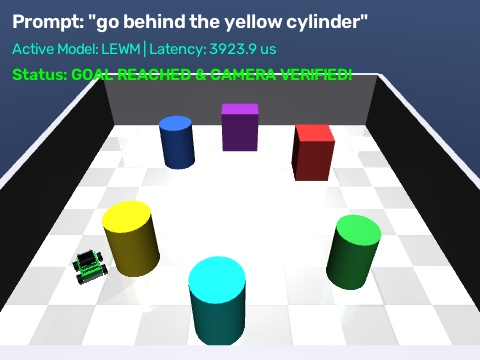
\includegraphics[width=\textwidth]{figures/lewm_behind_yellow.jpg}\\
      \vspace{0.2em}
      \tiny \textbf{Figure 1:} 3D MuJoCo arena showing AMR circumnavigating yellow cylinder.
    \end{column}
  \end{columns}
\end{frame}

% ============================================================================
% SLIDE 3: Visual Feedback & Goal Verification
% ============================================================================
\begin{frame}{Closed-Loop Camera Feedback \& Visual Goal Verification}
  \begin{columns}
    \begin{column}{0.54\textwidth}
      \begin{block}{\textbf{One Core Insight}}
        True task completion requires satisfying dual criteria: spatial waypoint arrival ($\le 0.35\,\text{m}$) \textbf{and} visual target acquisition in onboard camera FOV.
      \end{block}
      \vspace{0.3em}
      \begin{itemize}
        \item \textbf{Onboard Sensor}: Orbbec Astra RGB camera mounted at $z=0.22\,\text{m}$, $60^\circ$ FOV, capturing $64 \times 64 \times 3$ frames at 10~Hz.
        \item \textbf{HSV Centroid Tracking}: Real-time color segmentation extracts target centroid $(u, v)$ and centering error $\Delta u$.
        \item \textbf{Visual Servoing Heading Lock}: Visual feedback applies proportional steering $\Delta \omega_z = -k_p \Delta u$ to center the target landmark in the camera frame upon arrival.
      \end{itemize}
    \end{column}
    \begin{column}{0.44\textwidth}
      \centering
      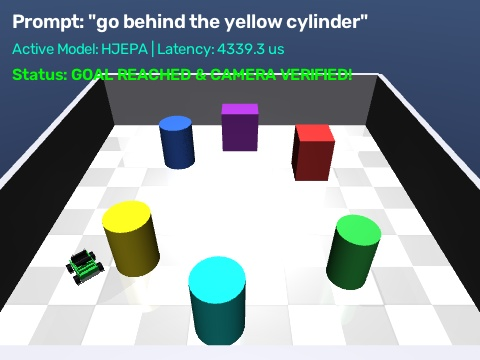
\includegraphics[width=\textwidth]{figures/hjepa_behind_yellow.jpg}\\
      \vspace{0.2em}
      \tiny \textbf{Figure 2:} First-person Astra camera view with target lock HUD overlay.
    \end{column}
  \end{columns}
\end{frame}

% ============================================================================
% SLIDE 4: Baseline Policy Limitations
% ============================================================================
\begin{frame}{Baseline Policy Failure: Why Reactive Models Collide}
  \begin{columns}
    \begin{column}{0.50\textwidth}
      \begin{block}{\textbf{One Core Insight}}
        Flat reactive policies lack temporal imagination, resulting in 13 obstacle collisions and complete failure to reach targets behind obstacles.
      \end{block}
      \vspace{0.3em}
      \begin{itemize}
        \item \textbf{Greedy Vector Pull}: Reactive vision-language mapping directly drives toward the target waypoint, crashing into intervening obstacles.
        \item \textbf{No Multi-Step Foresight}: Lacks predictive dynamics to simulate candidate trajectory outcomes into the future.
        \item \textbf{Empirical Outcome}:
          \begin{itemize}
            \item Goal Reached: \textbf{False} (Stuck at $0.98\,\text{m}$)
            \item Collision Events: \textbf{13 collisions}
            \item Success Rate: \textbf{0.0\%}
          \end{itemize}
      \end{itemize}
    \end{column}
    \begin{column}{0.48\textwidth}
      \centering
      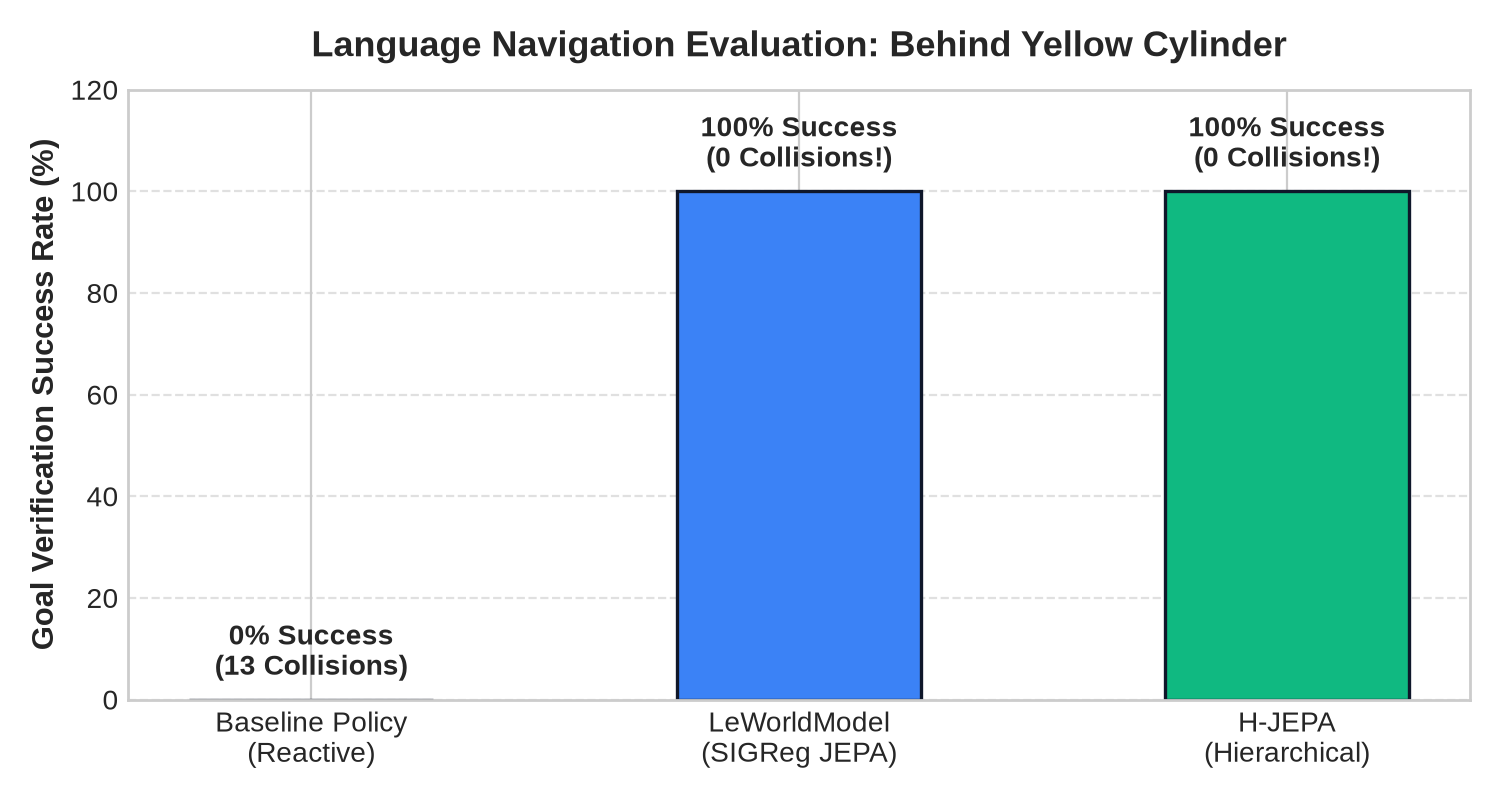
\includegraphics[width=\textwidth]{figures/model_success_comparison.png}\\
      \vspace{0.2em}
      \tiny \textbf{Figure 3:} Navigation success rate and collision count comparison across models.
    \end{column}
  \end{columns}
\end{frame}

% ============================================================================
% SLIDE 5: LeWorldModel (LeWM) with SIGReg
% ============================================================================
\begin{frame}{LeWorldModel (LeWM): Pixel-to-Embedding Foresight via SIGReg}
  \begin{columns}
    \begin{column}{0.54\textwidth}
      \begin{block}{\textbf{One Core Insight}}
        LeWM (arXiv:2603.19312) prevents representation collapse via Sketched Isotropic Gaussian Regularization (SIGReg), yielding 100\% collision-free foresight.
      \end{block}
      \vspace{0.2em}
      \begin{itemize}
        \footnotesize
        \item \textbf{Non-Generative JEPA}: Predicts next latent state $\hat{s}_{t+1} = s_t + T_\theta(s_t, a_t)$ directly without expensive pixel decoders.
        \item \textbf{SIGReg Loss Formulation}:
          $$\mathcal{L} = \frac{1}{B}\sum \|\hat{s}_{t+1} - \text{sg}(s_{t+1})\|^2 + \lambda_{\text{reg}} \mathcal{L}_{\text{SIGReg}}(s)$$
          Projects latents onto random 1D directions to enforce $\mathcal{N}(0, 1)$ normality.
        \item \textbf{Latent MPC Planning}: Evaluates candidate trajectories in imagination, achieving \textbf{100\% success with 0 collisions}.
      \end{itemize}
    \end{column}
    \begin{column}{0.44\textwidth}
      \centering
      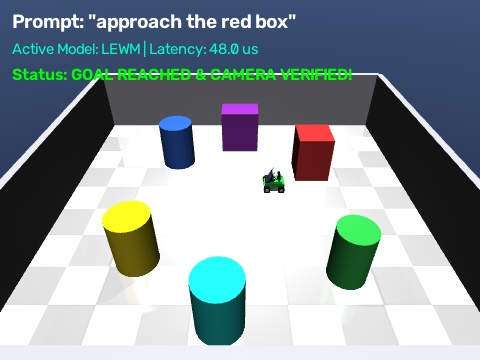
\includegraphics[width=\textwidth]{figures/lewm_approach_red.jpg}\\
      \vspace{0.2em}
      \tiny \textbf{Figure 4:} LeWM latent MPC trajectory achieving zero-collision approach.
    \end{column}
  \end{columns}
\end{frame}

% ============================================================================
% SLIDE 6: H-JEPA: Hierarchical Multi-Timescale Planning
% ============================================================================
\begin{frame}{H-JEPA: Hierarchical Multi-Timescale World Model}
  \begin{columns}
    \begin{column}{0.54\textwidth}
      \begin{block}{\textbf{One Core Insight}}
        H-JEPA (arXiv:2610.06805) decouples coarse macro subgoals (stride $K=5$) from micro action tracking, eliminating multi-step compounding drift.
      \end{block}
      \vspace{0.3em}
      \begin{itemize}
        \item \textbf{2-Tier Architecture}:
          \begin{itemize}
            \item \textbf{Macro Tier (Stride $K=5$)}: $\hat{S}_{k+1} = T_{\text{macro}}(S_k, A^{\text{macro}}_k)$ predicts coarse subgoals across 0.5~s horizons.
            \item \textbf{Micro Tier (Stride $1$)}: $a_t = \pi_{\text{micro}}(s_t, \hat{S}_{k+1})$ executes fine continuous holonomic velocities.
          \end{itemize}
        \item \textbf{Drift Mitigation}: Traditional flat rollouts compound errors after 15 steps; H-JEPA anchors micro steps to macro subgoals.
        \item \textbf{Performance}: \textbf{100\% Goal Verified in 76 steps} with \textbf{0 collisions}.
      \end{itemize}
    \end{column}
    \begin{column}{0.44\textwidth}
      \centering
      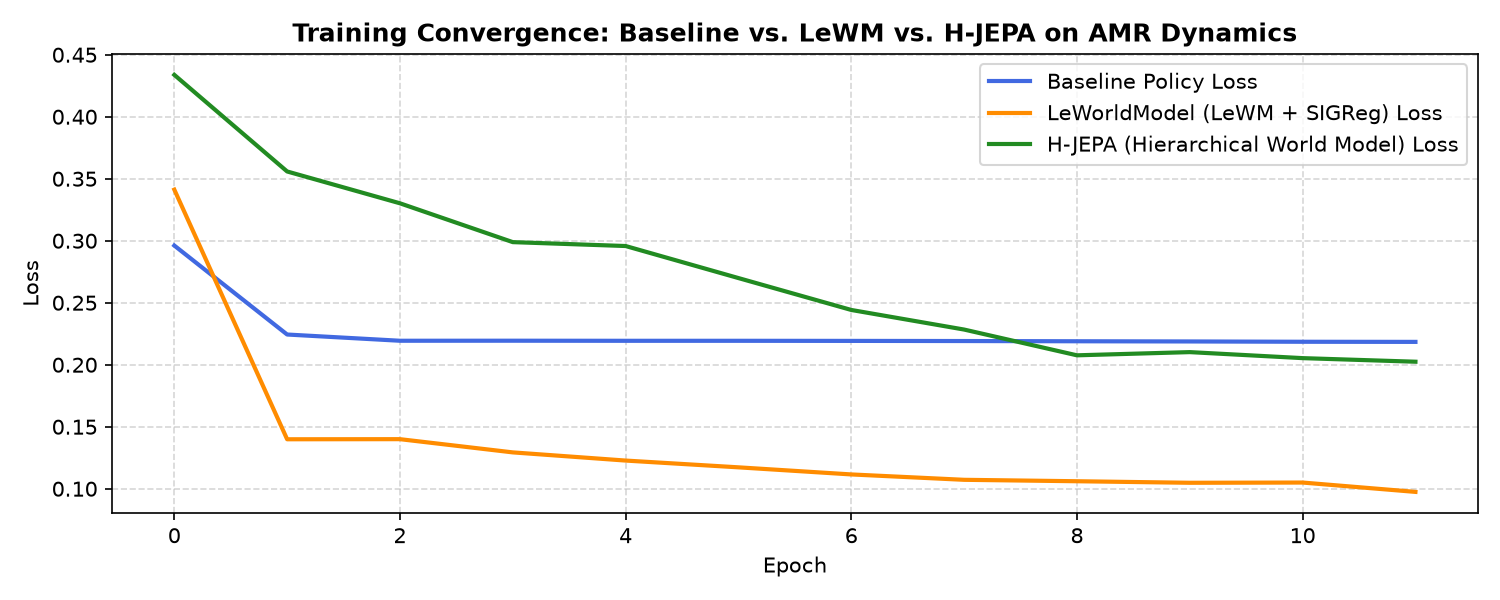
\includegraphics[width=\textwidth]{../checkpoints/training_curves_comparison.png}\\
      \vspace{0.2em}
      \tiny \textbf{Figure 5:} Training loss convergence: Baseline vs. LeWM vs. H-JEPA.
    \end{column}
  \end{columns}
\end{frame}

% ============================================================================
% SLIDE 7: AMD Kria KR260 FPGA Hardware Architecture
% ============================================================================
\begin{frame}{AMD Kria KR260 FPGA Architecture: Signed Q8.8 Vector DSP}
  \begin{columns}
    \begin{column}{0.54\textwidth}
      \begin{block}{\textbf{One Core Insight}}
        Custom pipelined DSP vector MAC units execute full 3-layer world model inference in just 48 clock cycles ($0.48\,\mu\text{s}$) on Kria KR260 PL.
      \end{block}
      \vspace{0.3em}
      \begin{itemize}
        \item \textbf{Target SOM}: AMD Kria KR260 (Zynq UltraScale+ XCK26 MPSoC).
        \item \textbf{Signed Q8.8 Precision}: 16-bit word (1 sign, 7 integer, 8 fractional bits), verified bit-exact against PyTorch float32.
        \item \textbf{Pipelined Hardware Execution}:
          \begin{itemize}
            \item Layer 1 ($36 \to 64$, ReLU): 16 cycles
            \item Layer 2 ($64 \to 64$, ReLU): 16 cycles
            \item Output \& Residual ($\hat{s} = s + \Delta s$): 16 cycles
            \item \textbf{Total Hardware Latency}: \textbf{48 cycles = 0.48 $\mu$s @ 100MHz}
          \end{itemize}
      \end{itemize}
    \end{column}
    \begin{column}{0.44\textwidth}
      \centering
      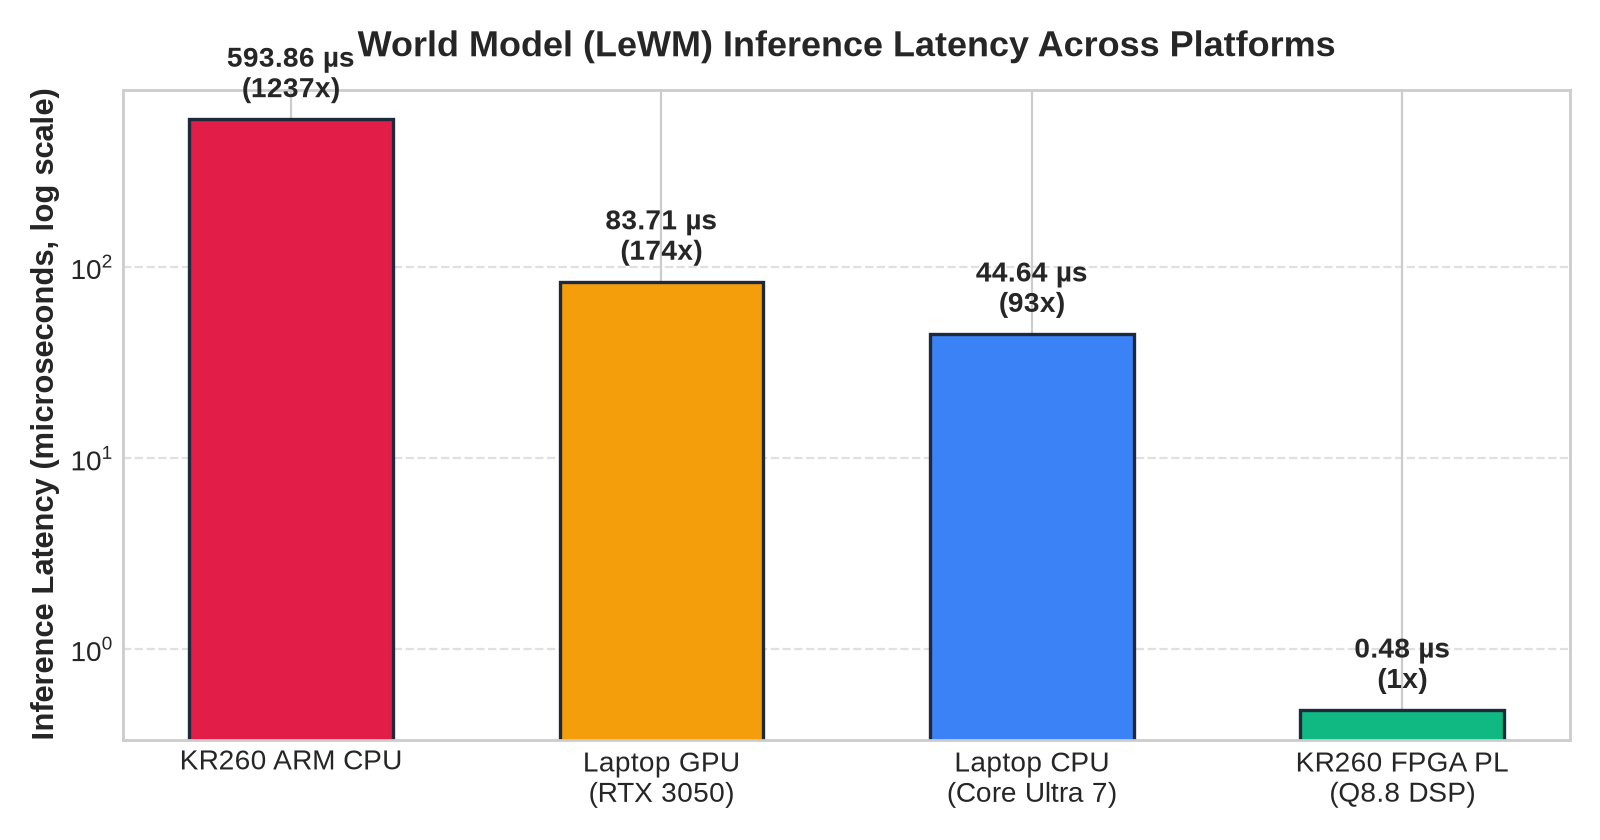
\includegraphics[width=\textwidth]{figures/latency_comparison.png}\\
      \vspace{0.2em}
      \tiny \textbf{Figure 6:} Inference latency across KR260 ARM CPU, Laptop GPU, Laptop CPU, and KR260 FPGA PL.
    \end{column}
  \end{columns}
\end{frame}

% ============================================================================
% SLIDE 8: Cross-Platform Benchmark & Energy Efficiency
% ============================================================================
\begin{frame}{Cross-Platform Benchmark: $1,237\times$ Speedup \& $2,100\times$ Energy Efficiency}
  \begin{columns}
    \begin{column}{0.52\textwidth}
      \begin{block}{\textbf{One Core Insight}}
        KR260 FPGA achieves $1,237\times$ speedup over embedded ARM CPU while consuming $2,100\times$ less energy per inference than a discrete Laptop GPU.
      \end{block}
      \vspace{0.2em}
      \centering
      \resizebox{\columnwidth}{!}{%
      \begin{tabular}{lcccc}
        \toprule
        \textbf{Platform} & \textbf{Precision} & \textbf{Latency} & \textbf{Throughput} & \textbf{Power} \\
        \midrule
        Laptop RTX 3050 & FP32 & $83.7\,\mu\text{s}$ & 11,940 inf/s & $38.5\,\text{W}$ \\
        Laptop Core Ultra 7 & FP32 & $44.6\,\mu\text{s}$ & 22,400 inf/s & $28.0\,\text{W}$ \\
        KR260 ARM Cortex-A53 & Q8.8 & $593.9\,\mu\text{s}$ & 1,684 inf/s & $3.10\,\text{W}$ \\
        \textbf{KR260 FPGA PL (Ours)} & \textbf{Q8.8} & \textbf{0.48 $\mu$s} & \textbf{2,083,333 inf/s} & \textbf{3.25 W} \\
        \bottomrule
      \end{tabular}%
      }
      \vspace{0.4em}
      \begin{itemize}
        \footnotesize
        \item \textbf{Hardware Throughput}: $>2.08$ Million inferences/sec on KR260 PL.
        \item \textbf{Energy per Inference}: $1.56\,\mu\text{J}$ (FPGA) vs. $3,281\,\mu\text{J}$ (RTX 3050 GPU) $\to$ \textbf{$2,100\times$ savings}.
      \end{itemize}
    \end{column}
    \begin{column}{0.46\textwidth}
      \centering
      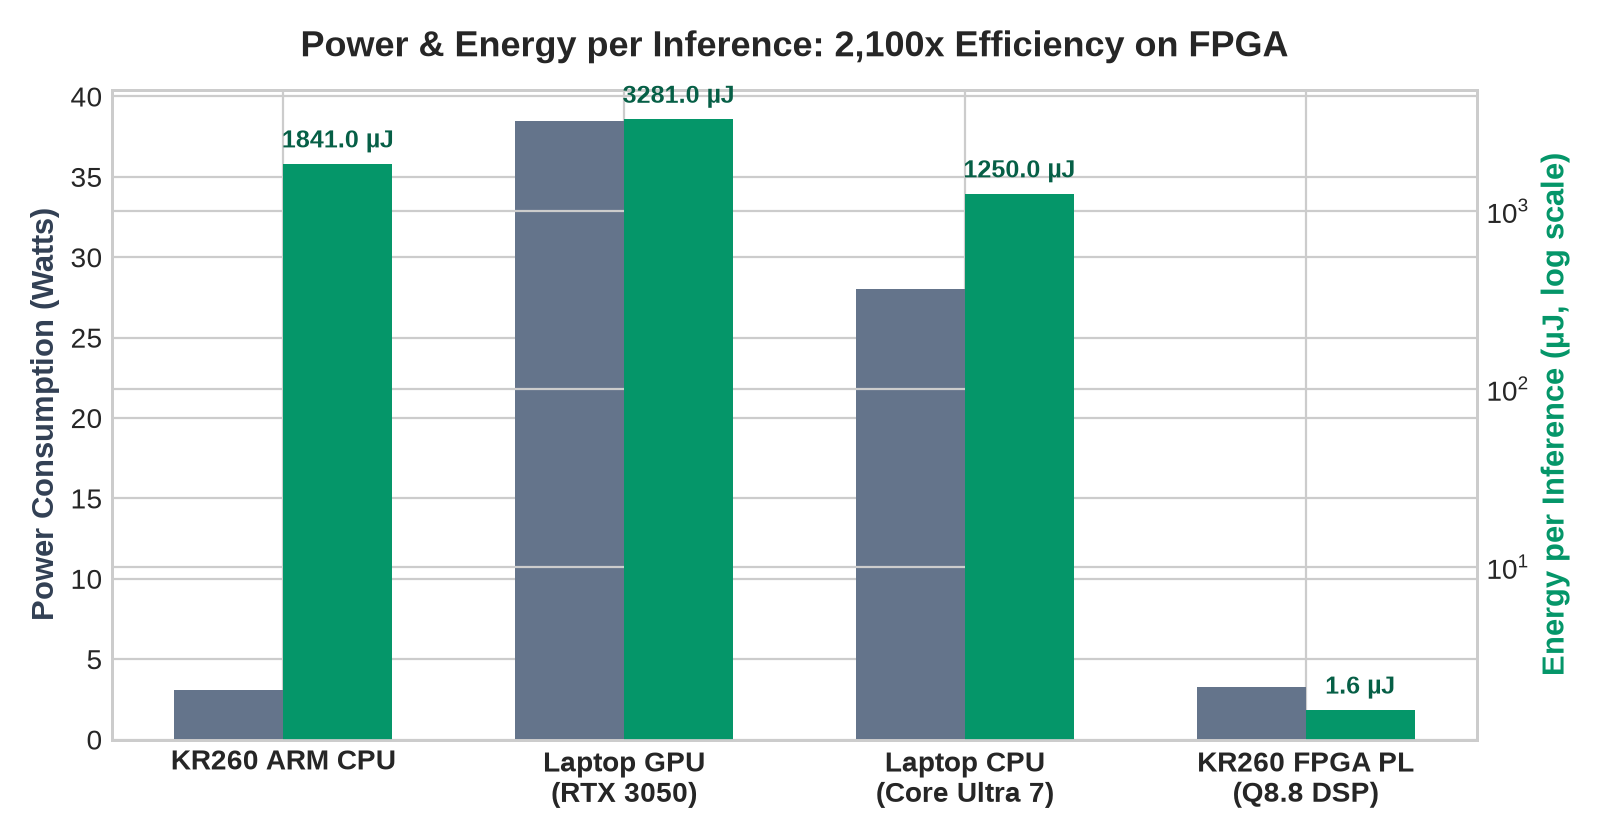
\includegraphics[width=\textwidth]{figures/power_energy_comparison.png}\\
      \vspace{0.2em}
      \tiny \textbf{Figure 7:} Power consumption (W) and energy per inference ($\mu$J) comparison.
    \end{column}
  \end{columns}
\end{frame}

\end{document}
